\documentclass[a4paper,12pt]{article}

\usepackage{amsmath,amssymb,multicol,tikz,enumitem}
\usepackage[margin=2cm]{geometry}
%\usetikzlibrary{calc}
\usepackage{amsmath}
\usepackage{amsthm}
\usepackage{thmtools}
\usepackage{hyperref}
\usepackage{enumerate}
\usepackage{xcolor}
\usepackage{fancyvrb}

\pagestyle{empty}

\newcommand\Q{\mathbf{Q}}
\newcommand\R{\mathbf{R}}
\newcommand\Z{\mathbf{Z}}

\newcommand\answer[1]{}
\newcommand\ans[1]{}
%\newcommand\answer[1]{\\[5pt]{\color{blue}{#1}}\hfill{\color{blue}}\\[-5pt]}
%\newcommand\ans[1]{{\color{blue}{#1}}}

\usepackage{array}
\newcolumntype{P}[1]{>{\centering\arraybackslash}p{#1}}

\newcommand\indd{${}$\hspace{20pt}}

\declaretheoremstyle[headfont=\normalfont\bfseries,notefont=\mdseries\bfseries,bodyfont = \normalfont,headpunct={:}]{normalhead}
\declaretheorem[name={Uzdevums}, style=normalhead,numberwithin=section]{problem}

\setcounter{section}{05}

\setlength\parindent{0pt}

\renewcommand{\figurename}{Attēls}

\begin{document}

\begin{center}
\parbox{3.5cm}{\flushleft\bf Dažāda skaitļu teorija} \hfill {\bf\LARGE Sacensības \#2021.05} \hfill \parbox{3.5cm}{\flushright\bf 2021-04-29} \\[2pt]
{\rm\footnotesize Par šo LU NMS atbalstīto pasākumu\\ atbild {\tt kalvis.apsitis@gmail.com}.}
\end{center}

%\hrule\vspace{2pt}\hrule
\hrule

%%%%%%%%%%%%%%%
%%% 01 %%%%%%%%
%%%%%%%%%%%%%%%
\vspace{10pt}
\begin{problem}
%2021.2.9
Atrast, cik ir sakārtotu pāru ar naturāliem skaitļiem $(m,n)$,
ka $m,n \in \{ 1,2,\ldots,64 \}$ un lielākais kopīgais 
dalītājs $\text{LDK}(2^m + 1, 2^n - 1) > 1$. 
\answer{

{\bf Atbilde.} $\mathtt{1365}$

Visiem nepāra $m$, $2^m + 1$ dalās ar $3$. Tāpēc veido derīgu pāri ar jebkuru pāra skaitli $n$ (kam savukārt $2^n - 1$ dalās ar $3$). 
Šādu pāru ir pavisam $32 \cdot 32 = 1024$. 

Visiem pāra $m$ (kas nedalās ar $4$), $2^m + 1$ dalās ar $5$. Tie veido derīgu pāri ar jebkuru $n$, kas dalās ar $4$. 
Šādu pāru ir pavisam $16 \cdot 16 = 256$. 

Visiem pāra $m$ (kas dalās ar $4$, bet nedalās ar $8$), $2^m + 1$ dalās ar $17$. Tie veido derīgu pāri ar jebkuru $n$, kas dalās ar $4$. 
Šādu pāru ir pavisam $8 \cdot 8 = 64$. Utt. 

Visbeidzot $m = 32$ veido pāri tikai ar $n = 64$ (var pārbaudīt dalāmību, izmantojot kvadrātu starpības formulu).

\[ 32 \cdot 32 + 16 \cdot 16 + 8 \cdot 8 + 4 \cdot 4 + 2 \cdot 2 + 1 \cdot 1 = 1365. \]

}
\end{problem}


%%%%%%%%%%%%%%%
%%% 02 %%%%%%%%
%%%%%%%%%%%%%%%
\vspace{10pt}
\begin{problem}
%2021.2.11
Skolotājs iedomājās skaitļu kopu $S$ no četriem skaitļiem; 
katru skaitli no kopas $S$ viņš iečukstēja ausī vienam no četriem skolēniem. 
Tad skolotājs visiem skaļi pateica, ka tie ir četri pēc kārtas 
sekojoši divciparu skaitļi; ka vismaz viens no tiem dalās ar $6$, bet
kāds cits šīs kopas skaitlis dalās ar $7$. 
Viņš jautāja skolēniem, vai viņi var nosaukt visus skaitļus no kopas $S$
un skolēni (kuri vienmēr runā patiesību un izdara pareizus 
loģiskus secinājumus) visi korī atbildēja ``Nē''.

Tomēr, tiklīdz kā viņi bija dzirdējuši cits cita atbildes, 
katrs no viņiem jau varēja pateikt visus 
kopas $S$ elementus: $S = \{ s_1,s_2,s_3,s_4 \}$.
Atrast visu iespējamo $s_1$ summu (ar $s_1$ apzīmē $S$ mazāko elementu).

{\bf Jautājums.} Ierakstīt atbildē naturālu skaitli: Visu iespējamo $s_1$ summu.
\answer{

{\bf Atbilde.} $\mathtt{246}$

Skaitļiem, kuri dalās ar $6$ un $7$ jāatrodas skaitļu ``četrinieka'' vidū (ja kāds atrodas malā, tad
tas, kurš atrodas otrā malā, var uzreiz uzminēt).

Atrodam visus četrus $7$ daudzkārtņus, kas ir blakus $6$ daudzkārtnim: $\{ 35,  49, 77, 91 \}$ ($6$ daudzkārtņi ir attiecīgi $36, 48, 78, 90$).\\
Mazākie skaitļi šajās kopās ir šādi: $34, 47, 76, 89$. To summa ir $246$.
}
\end{problem}


%x <- (7*(15:142))
%# Atrod un summē visus skaitļa 7 daudzkārtņus, 
%#   kas ir blakus skaitlim, kas dalās ar 6.
%sum(x[which(x %% 6 == 1 | x %% 6 == 5)])







%%%%%%%%%%%%%%%
%%% 03 %%%%%%%%
%%%%%%%%%%%%%%%
\vspace{10pt}
\begin{problem}
%2021.2.3
Ar $x_1,x_2,x_3,x_4,x_5,x_6$ apzīmējam skaitļu $1,2,3,4,5,6$ permutāciju
(katrs skaitlis ir piešķirts vienam no mainīgajiem; visu mainīgo 
vērtības ir dažādas). 
Atrast, cik ir tādu permutāciju, kurām sekojoša izteiksme
dalās ar $3$: 
\[ x_1x_2x_3 + x_2x_3x_4 + x_3x_4x_5 + x_4x_5x_6 + x_5x_6x_1 + x_6x_1x_2. \]
\answer{

{\bf Atbilde.} $\mathtt{336}$.

Uzrakstām visus permutācijas elementus uz apļa kā Attēlā~\ref{fig:q4-circles}.
Der visi tie izvietojumi, kuros abas vērtības, kas dalās ar $3$ ($3$ un $6$) atrodas
pretī viena otrai (jo tad visi saskaitāmie arī dalās ar $3$). 
Šādu izvietojumu ir $6 \cdot 1 \cdot 4 \cdot 3 \cdot 2 \cdot 1$ (pirmo skaitli ``$3$'' izvēlas vienā 
no sešām vietām; tad skaitļa ``$6$'' atrašanās vieta ir tikai viena iespējamā; pēc tam $1,2,4,5$ novieto 
pārpalikušajās $4$ vietās $4!$ dažādos veidos.

\begin{figure}[!htb]
\center{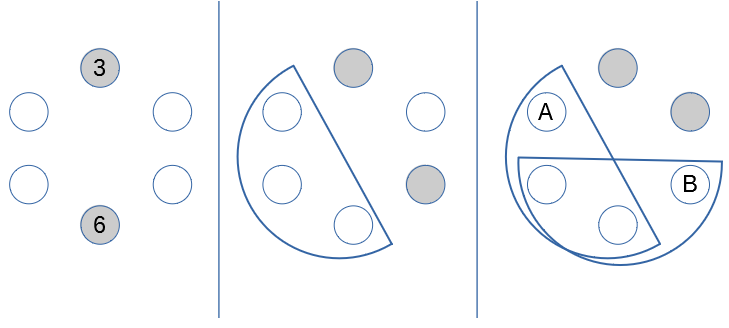
\includegraphics[width=4in]{online-competition-2021-04-29/q4-circles.png}}
\caption{\label{fig:q4-circles} Trīs gadījumi atkarībā no skaitļu $3$ un $6$ savstarpējā novietojuma.}
\end{figure}

Tie izvietojumi, kur starp $3$ un $6$ ir viens skaitlis, neder (jo tad
izteiksmē ir tieši viens saskaitāmais, kurš nedalās ar $3$). Tas redzams vidējā
sadaļā Attēlā~\ref{fig:q4-circles}, kur skaitļu $3$ un $6$ aplīši ir iekrāsoti pelēki.

Visbeidzot, izvietojumi, kur $3$ un $6$ atrodas blakus, der tad un tikai tad, ja
skaitļi, kuri ir blakus attiecīgi skaitļiem ``$3$'' un ``$6$'' nav savstarpēji kongruenti pēc moduļa $3$. 
Attēla~\ref{fig:q4-circles} labajā daļā $A \not\equiv B \pmod{3}$. 
Tikai šajā gadījumā divi saskaitāmie, kuri nedalās ar $3$, summā dos skaitli, kas dalās ar $3$). 
Tādu izvietojumu pavisam ir $6 \cdot 2 \cdot 4 \cdot 2 \cdot 2 \cdot 1$ (vispirms novietojam ``$3$'' kādā no sešām 
vietām; pēc tam novietojam skaitli ``$6$'' tam vienā vai otrā pusē - var izdarīt divos veidos; 
pēc tam patvaļīgi izvēlas otru skaitļa ``$3$'' kaimiņu (četros veidos); tad izvēlas otru skaitļa ``$6$'' 
kaimiņu (divos veidos, jo tas nav kongruents ar iepriekšējā solī izvēlēto). 
Visbeidzot, $2!$ veidos aizpilda atlikušās divas vietas.

Iegūstam summu: $6 \cdot 1 \cdot 4 \cdot 3 \cdot 2 \cdot 1 + 6 \cdot 2 \cdot 4 \cdot 2 \cdot 2 \cdot 1 = 336$.
}
\end{problem}




%%%%%%%%%%%%%%%
%%% 04 %%%%%%%%
%%%%%%%%%%%%%%%
\vspace{10pt}
\begin{problem}
%2004.2.8
Cik daudzi pozitīvie skaitļa $2021^{2021}$ dalītāji ir tādi, kuriem 
pašiem ir tieši $2021$ pozitīvi dalītāji?
\answer{

{\bf Atbilde.} $\mathtt{4}$.

Sadalām pirmreizinātājos: $2021 = 43 \cdot 47$. Skaitļa $2021^{2021}$ 
visi dalītāji būs formā $43^a \cdot 47^b$. 

Meklējam skaitļus ar tieši $2021$ (nepāra skaitu) dalītāju kā pilnus kvadrātus: $d = 43^{2m}47^{2n}$, kur 
abi pirmreizinātāji kāpināti pāra pakāpēs.
Šādiem skaitļiem visu dalītāju skaits ir $(2m+1)(2n+1)$; prasām, lai šis reizinājums būtu tieši $2021$. 
Šo reizinājumu var iegūt četros veidos: $1 \cdot 2021 = 43 \cdot 47 = 47 \cdot 43 = 2021 \cdot 1$. 

Atbilstošie skaitļa $2021^{2021}$ dalītāji (katram no kuriem ir tieši $2021$ pozitīvi dalītāji) 
ir $43^{0}\cdot{}47^{2020}$, $43^{42}\cdot{}47^{46}$, $43^{46}\cdot{}47^{42}$, $43^{2020}\cdot{}47^{0}$.
}
\end{problem}


%%%%%%%%%%%%%%%
%%% 05 %%%%%%%%
%%%%%%%%%%%%%%%
\vspace{10pt}
\begin{problem}
%2003.1.13
Ar $N$ apzīmējam naturālo skaitļu skaitu, kas nepārsniedz $2021$ un 
kuru binārajā pierakstā ir vairāk ciparu {\tt 1} nekā ciparu {\tt 0}. 
Atrast skaitli $N$.
\answer{

{\bf Atbilde.} $\mathtt{1173}$

Pierakstām skaitli $2021$ binārajā pierakstā: 
\[ 2021_{10} = 1024 + 512 + 256 + 128 + 64 + 32 + 0\cdot{}16 + 0\cdot{}8 + 4 + 0\cdot2 + 1 = 11111100101_{2}. \]
Visiem turpmākajiem skaitļiem līdz pat $2^{11} -1 = 2047$ būs vieninieku pārsvars pār nullēm (jo arī tiem skaitļa pieraksts sākas ar vismaz sešiem vieniniekiem). 

Tāpēc vispirms saskaitīsim, cik ir skaitļu, kuros ir vairāk ciparu {\tt 1} nekā ciparu {\tt 0} no skaitļa $1$ līdz pat $2047$. 
To skaits redzams Attēlā~\ref{fig:pascal-triangle} attēlotajā Paskāla trijstūrī (pa labi no sarkanās robainās līnijas). 

\begin{figure}[!htb]
\center{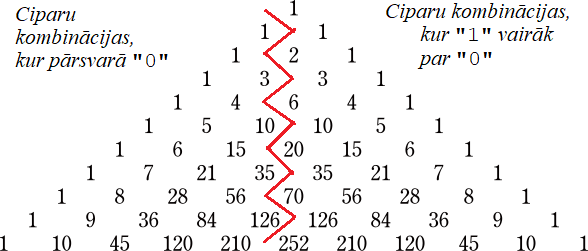
\includegraphics[width=4in]{online-competition-2021-04-29/pascal-triangle.png}}
\caption{\label{fig:pascal-triangle} Paskāla trijstūris ar kombinācijām, kurās {\tt 1} vairāk nekā {\tt 0}.}
\end{figure}

Tie skaitļi, kuru binārais pieraksts satur $k$ ciparus (no kuriem pirmais vienmēr ir {\tt 1}) atbilst Paskāla 
trijstūra $(k-1)$-tajai rindiņai. 
Piemēram, ir $6 + 4 + 1 = 11$ dažādi $5$-ciparu skaitļi, kuros vieninieku skaits pārsniedz nuļļu skaitu: 
\begin{itemize}
\item $C_4^2 = 6$ skaitļi, kur pirmajam vieniniekam seko 
kombinācija ar diviem vieniniekiem un divām nullēm: {\tt 10011}, {\tt 10101}, {\tt 10110}, {\tt 11001}, {\tt 11010}, {\tt 11100}.
\item $C_4^3 = 4$ skaitļi, kur pirmajam vieniniekam seko kombinācija ar
trim vieniniekiem un vienu nulli: {\tt 11110}, {\tt 11101}, {\tt 11011}, {\tt 10111}. 
\item $C_4^4 = 1$ skaitlis, kur pirmajam vieniniekam seko vēl četri vieninieki: {\tt 11111}.
\end{itemize}


Zinot to, ka $n$-tajā Paskāla trijstūra rindiņā kombināciju summa ir $2^n$, iegūstam šādu izteiksmi:
\[ \frac{1}{2} \cdot \left( 2^0 + 2^1 + 2^2 + \ldots + 2^{10} \right) + \frac{1}{2} \cdot \left( 1 + 2 + 6 + 20 + 70 + 252 \right) = 1199. \]
Ņemot vērā to, ka esam ieskaitījuši arī visus skaitļus no $2022$ līdz $2047$ (abus galapunktus ieskaitot), jāatņem $(2047 - 2022) + 1 = 26$. 

Iegūstam $1199 - 26 = 1173$.
}
\end{problem}




%%%%%%%%%%%%%%%
%%% 06 %%%%%%%%
%%%%%%%%%%%%%%%
\vspace{10pt}
\begin{problem}
%1992.15
Sauksim skaitli $n$ par {\em faktoriāla asti}, ja eksistē kāds naturāls $m$, 
kuram $m!$ decimālpieraksts beidzas  ar tieši $n$ nullēm. 
Cik daudzi naturāli skaitļi no intervāla $[1;2021]$ {\bf nav} faktoriālu astes?
\answer{


{\bf Atbilde.} $\mathtt{402}$.

Ievērojam, ka nuļļu skaits faktoriāla $n!$ beigās atkarīgs no lielākās skaitļa $5$ pakāpes, 
ar kuru dalās $n!$ (jo katra nulle veidojas, sareizinot pirmreizinātāju $2$ ar pirmreizinātāju $5$
un skaitļa $2$ pakāpe, ar kuru dalās $n!$ aug straujāk nekā skaitļa $5$ pakāpe). 

Ar $\nu_5(m)$ apzīmēsim skaitļa $m$ ``$5$-valuāciju'' \textendash{} lielāko kāpinātāju $k$, 
pie kura $m$ dalās ar $5^k$. Ir spēkā Ležandra formula, kas izsaka valuāciju jebkuram faktoriālam: 
\[ \nu_5(n!) = \sum\limits_{i=1}^{\infty} \left\lfloor \frac{n}{5^i} \right\rfloor = \left\lfloor \frac{n}{5} \right\rfloor +
\left\lfloor \frac{n}{25} \right\rfloor + \left\lfloor \frac{n}{125} \right\rfloor + \left\lfloor \frac{n}{625} \right\rfloor + \ldots. \]

Risinām vienādojumu: 
\begin{equation} 
\label{eq:legendre2021}
f(n) := \left\lfloor \frac{n}{5} \right\rfloor +
\left\lfloor \frac{n}{25} \right\rfloor + \left\lfloor \frac{n}{125} \right\rfloor + \left\lfloor \frac{n}{625} \right\rfloor + 
\left\lfloor \frac{n}{3125} \right\rfloor = 2021. 
\end{equation}

Summa $n/5 + n/25 + n/125 + n/625 + n/3125 \approx n/4$ ir aptuveni ģeometriskā 
progresija, kas tiecas uz $n/4$; tāpēc $n$ būs tuvs $2021 \cdot 4$
(ja ignorē noapaļošanu uz leju 
veselajās daļās $\lfloor \ldots \rfloor$). Bet, ievietojot $n = 8084$ 
izteiksmē (\ref{eq:legendre2021}), iegūstam $f(8084) = 2017$, t.i. 
$n$ vajag palielināt apmēram par $4 \cdot 4 = 16$. 

Izrādās, ka vienādojumu (\ref{eq:legendre2021}) neapmierina neviens skaitlis, 
jo $f(8095) = 2020$, bet $f(8100) = 2022$ (t.i.\ $8100!$ beidzas jau ar $2022$ nullēm)
un skaitlis $2021$ {\bf nav} faktoriāla aste.

Pavisam pirms vērtības $f(8100) = 2022$ ir $8100/5 =1620$ {\bf atšķirīgas}
faktoriāla astes (jo ikreiz, kad $n$ dalās ar $5$, astes garums
pieaug vismaz par vienu jaunu nulli). Atmetam skaitli $0 \not\in [1;2021]$ (daži pirmie faktoriāli vispār nebeidzas ar nullēm), 
tātad  naturālās astes, kuras nepārsniedz $2021$ ir tieši $1619$.

 
Tātad tieši $2021 - 1619 = 402$ skaitļi nebūs faktoriālu astes
(tiem pārlēks pāri pateicoties tam, ka $n$ dalās ar $25$, $125$ vai vēl 
augstāku $5$ pakāpi). 
}
\end{problem}



%%%%%%%%%%%%%%%
%%% 07 %%%%%%%%
%%%%%%%%%%%%%%%
\vspace{10pt}
\begin{problem}
%1990.5
Ar $n$ apzīmējam mazāko naturālo skaitli, kas dalās ar $75$ un kam ir 
tieši $75$ naturāli dalītāji (ieskaitot $1$ un pašu skaitli). 
Atrast šo skaitli $n$. 
\answer{

{\bf Atbilde.} $\mathtt{32400}$.

Ievērojam, ka $75$ ir nepāra skaitlis; tāpēc skaitlis $n$ ar šādu dalītāju 
skaitu ir pilns kvadrāts (visi tā pirmreizinātāji tiek kāpināti pāra pakāpēs). 

Skaitlim $n$ ir vismaz divi dažādi pirmreizinātāji ($3$ un $5$), citādi tas nedalīsies ar $75$.  
Bet tam varētu būt arī trīs dažādi pirmreizinātāji: $n = 3^{2a}5^{2b}2^{2c}$ 
(izvēlēties skaitļa $2$ vietā pirmskaitli $p \geq 7$ nav optimāli, jo dalītāju skaits 
nemainīsies, bet skaitlis $n$ kļūs lielāks). 

Aplūkosim vispirms $3$ pirmreizinātāju gadījumu, jeb $n = 3^{2a}5^{2b}2^{2c}$.\\
Tad skaitļa $n$ dalītāju skaitu var izteikt kā $(2a+1)(2b+1)(2c+1)$, kas vienāds ar $75$. 
Iegūstam, ka divi no mainīgajiem $a,b,c$ vienādi ar $2$, bet viens vienāds ar $1$, lai 
$(2\cdot 2 + 1)(2\cdot 2 + 1)(2\cdot 1 + 1) = 75$. Mazāko kāpinātāju lietosim lielākajam 
pirmskaitlim $5$. Tātad, der atbilde $n = 2^4 3^4 5^2 = 32400$, kas arī ir optimālā atbilde.

Skaitlim $n$ nevar būt vairāk kā $3$ pirmreizinātāji (visi pāra pakāpēs, jo $n$ ir pilns kvadrāts). 
Jo citādi, piemēram, $(2a+1)(2b+1)(2c+1)(2d+1)$ (četru nepāra skaitļu $>1$ reizinājums) pārsniegtu $75$. 

Nav arī izdevīgi, ja skaitlim $n$ ir tikai divi pirmreizinātāji, jo tad jāizvēlas $n = 3^{2a}5^{2b}$, 
un $(2a+1)(2b+1) = 75$. Vismaz viena no iekavām (piemēram $2a+1$ ir vismaz $15$ (jo $15 \cdot 5 = 75$). 
Bet tad $3^{14}$ jau pārsniedz $32400$, ko atradām iepriekš (vēl jo vairāk, ja to pareizinās ar kādu 
skaitļa $5$ pakāpi). Tāpēc optimālā atbilde ir $n=32400$, kam vajag trīs pirmreizinātājus.
}
\end{problem}



%%%%%%%%%%%%%%%
%%% 08 %%%%%%%%
%%%%%%%%%%%%%%%
\vspace{10pt}
\begin{problem}
%1987.11
Atrast lielāko iespējamo $k$ vērtību, kurai 
$6^{6}$ var izteikt kā $k$ pēc kārtas sekojošu naturālu skaitļu summu. 
\answer{

{\bf Atbilde.} $\mathtt{243}$.

Pie $k = 243$ var sasummēt $71 + 72 + \ldots + 312 + 313 = 46656$. 
(Šajā progresijā vidējais loceklis ir $6^6/243 = 192$ un no tā var izrēķināt visus pārējos.)

{\em Piezīme.} Lai stingri pamatotu, ka nekā labāka nav, jāaplūko arī dažas pāru atbildes (piemēram $k = 128$, jo 
var summēt $301 + \ldots + 428 = 46656 = 6^6$). 
Bet tās šoreiz nav optimālas. 
}
\end{problem}


%%%%%%%%%%%%%%%
%%% 09 %%%%%%%%
%%%%%%%%%%%%%%%
\vspace{10pt}
%\clearpage
\begin{problem}
%EGMO2016.Q6
%2   12   70  408 2378
%6   84 1170
\[ \left\{ \begin{array}{l}
\sqrt{2 \cdot 8} = 4 = n^2,\\
(2 + 8)/2 = 5 = n^2+1.\\
\end{array} \right. \]
\[ \left\{ \begin{array}{l}
\sqrt{27 \cdot 48} = 36 = n^2,\\
(27 + 48)/2 = 37.5 = n^2+1.5.\\
\end{array} \right. \]
\[ \left\{ \begin{array}{l}
\sqrt{128 \cdot 162} = 144 = n^2,\\
(128 + 162)/2 = 145 = n^2+1.\\
\end{array} \right. \]
\[ \left\{ \begin{array}{l}
\sqrt{4802 \cdot 5000} = 4900 = n^2,\\
(4802 + 5000)/2 = 4901 = n^2+1.\\
\end{array} \right. \]
Attēlā redzamajos piemēros ir vairākas $n$ vērtības ($n = 2,6,12,70$), 
kurām eksistē divi naturāli $a,b$, kuru vidējais ģeometriskais $\sqrt{ab}$
ir $n^2$, bet vidējais aritmētiskais ir par $1$ vai par $1.5$
lielāks nekā $n^2$. 

Atrast vēl kādu $n$ vērtību (divciparu vai trīsciparu skaitli) ar 
šādu īpašību. 
\answer{

{\bf Atbilde.} $\mathtt{84}$ vai $\mathtt{408}$. 

Var pārbaudīt vienādības: 
\[ \left\{ \begin{array}{l}
\sqrt{6912 \cdot 7203} = 7056 = 84^2,\\
(6912 + 7203)/2 = 7057.5 = 84^2+1.5.\\
\end{array} \right. \]
Kā arī 
\[ \left\{ \begin{array}{l}
\sqrt{165888 \cdot 167042} = 166464 = 408^2,\\
(165888 + 167042)/2 = 166465 = 408^2+1.\\
\end{array} \right. \]
Tās vērtības $n$, kurām $\sqrt{ab} = n^2$ un $(a+b)/2 = n^2 + 1$ apmierina
Pella vienādojumu $2n^2 + 1 = m^2$ (kaut kādam veselam $m$). 
Pella vienādojums izskaidro, kāpēc attālumi starp atrisinājumiem strauji pieaug.
}
\end{problem}



%%%%%%%%%%%%%%%
%%% 10 %%%%%%%%
%%%%%%%%%%%%%%%
\vspace{10pt}
\begin{problem}
%1985.13
Skaitļu virkni $501, 504, 509, 516, 525, \ldots$ veido pēc formulas $a_n = 500+n^2$ ($n = 1,2,3,\ldots$). 
Ar $d_n$ apzīmējam skaitļu $a_n$, $a_{n+1}$ lielāko kopīgo dalītāju. 
Atrast $d_n$ maksimumu, ja $n$ pieņem visas iespējamās vērtības no naturālo skaitļu kopas.
\answer{

{\bf Atbilde.} $\mathtt{2001}$.

Izteiksmēm $500 + n^2$ un $500 + n^2 + 2n + 1$ lieto Eiklīda algoritmu, pēc vairākiem 
pārveidojumu soļiem iegūst $\text{LKD}(n-1000, 2001)$.

}
\end{problem}


%%%%%%%%%%%%%%%
%%% 11 %%%%%%%%
%%%%%%%%%%%%%%%
\vspace{10pt}
\begin{problem}
%EGMO2013.Q4
Kādam naturālam skaitlim $b>1$ ir definēts polinoms 
\[ P(x) = \frac{1}{b} x^5 + \frac{1}{b}, \] 
kurš trim pēc kārtas sekojošiem naturāliem skaitļiem pieņem 
naturālas vērtības: $P(n)$, 
$P(n+1)$ un $P(n+2)$. 

Atrast polinomu (ievietot tajā derīgu parametru $b$), kas izpilda šo īpašību un atrast mazāko $n$, kam $P(n)$, $P(n+1)$ un 
$P(n+2)$ ir naturāli skaitļi.

{\bf Jautājums.} Ierakstīt atbildē mazāko polinoma vērtību $P(n)$. (Tātad atbildē jānorāda vērtība, nevis arguments $n$.)
\answer{

{\bf Atbilde.} $\mathtt{707}$.

Var pamatot, ka vienīgā naturālā $b>1$ vērtība, kam trīs vērtības $x^5+1$ pēc kārtas dalās ar $b$ ir $b = 11$. 
Un jāievieto skaitļi $n = 6$, $n+1 = 7$, $n+2 = 8$. 
Ievietojot mazāko $n$, iegūstam: 
\[ (6^5 + 1) / 11 = 7777 / 11 = 707. \]
}
\end{problem}



%%%%%%%%%%%%%%%
%%% 12 %%%%%%%%
%%%%%%%%%%%%%%%
\vspace{10pt}
\begin{problem}
%1986.8
Ar $S$ apzīmējam visu logaritmu (ar logaritma bāzi $10$) summu skaitļiem, kuri 
ir skaitļa $1000000$ dalītāji. Kurš veselais skaitlis ir vistuvākais skaitlim $S$? 
\answer{

{\bf Atbilde.} $\mathtt{147}$.

Skaitlim $1000000 = 2^6 5^6$ dalītāju skaitu var atrast ar izteiksmi: 
\[ \sigma_0(1000000) = (1 + 6)\cdot (1 + 6) = 49. \]
Viens no dalītājiem ir $d = 1000$, kura logaritms ir $3$. 
Visi citi ir sadalāmi pa pāriem tā, ka $ab = 1000000$; 
tāpēc $\log_{10} a + \log_{10} b = 6$. Vidēji jāpieskaita $3$ uz katru dalītāju. 

Visu šo logaritmu summa būs $3 \cdot 49 = 147$. 
}
\end{problem}




\end{document}









